\begin{answer}

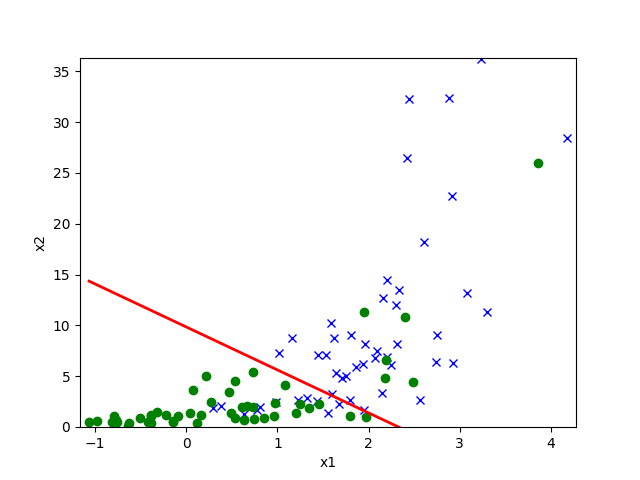
\includegraphics[width=0.5\textwidth]{linearclass/logreg_plot_1_valid.png}
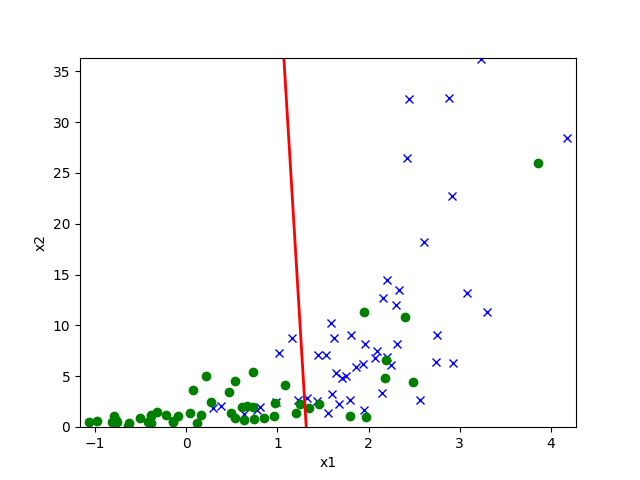
\includegraphics[width=0.5\textwidth]{linearclass/gda_plot_1_valid.png}

Logistic regression (left), GDA (right)

In logistic regression, they find the boundary which loss of train is as less as possible. Contrarily GDA assume the distributions are gaussian then find the center points of $y=1$ and $y=0$ respectively. Therefore, boundary of logistic regression is made by only data, and boundary of GDA is middle line of two center points. In this dataset, the distributions do not look like gaussian. This is why two boundaries aren't same.

\end{answer}
